\chapter{Werkzeuge}
\label{chap:tools}

%%%%%%%%%%%%%%%%%%%%%%%%%%%%%%%%%%%%%%%%%%%%%%%%%%%%%%%%%%%%
\section{Xcode}
\label{sec:tools:xcode}
%%%%%%%%%%%%%%%%%%%%%%%%%%%%%%%%%%%%%%%%%%%%%%%%%%%%%%%%%%%%
Xcode ist eine integrierte Entwicklungumgebung von Apple, welche es ermöglicht iOS und OS X Applikationen zu programmieren, zu testen und zu debuggen.
Standardmäßig werden dabei die Programmiersprachen \emph{Objective C}, \emph{C} und \emph{C++} unterstützt.

Xcode stellt viele Features für die Programmierung bereit, wie zum Beispiel \emph{code completion}, vorgefertigte \emph{Templates}, einen umfangreichen \emph{Debugger} und eine \emph{iOS-Simulator} für das Testen der Applikationen.

Bei Erstellung einer neuen Applikation kann man unter mehreren Templates wählen, welche jeweils verschiedene Funktionen mit sich bringen. In Abbildung \ref{xcode-templates} lassen sich die verschiedenen Auswahlmöglichkeiten erkennen.

\begin{figure}[htb!]
		\centering
	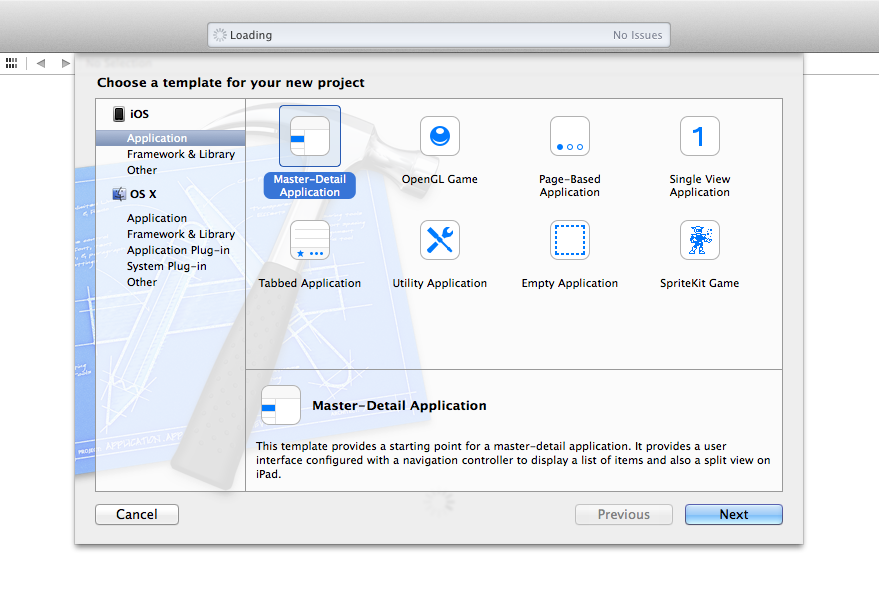
\includegraphics[scale=0.4]{xcode-templates}
	\caption{Auswahlbildschirm der verschiedenen Templates}
	\label{xcode-templates}
\end{figure}

Nach dem man das passende Template gewählt hat, werden die benötigten Dateien angelegt.
Dazu gehören beispielsweise die \emph{AppDelegate} und das \emph{Storyboard}.

Die AppDelegate-Klasse steuert applikationsweite Ereignisse, wie etwa das Aufrufen und Schließen der Applikation. Außerdem wird durch die AppDelegate der aktuelle Zustand der Applikation gespeichert und wiederhergestellt.

Das Storyboard ist eine grafische Oberfläche für die Erstellung des User Interfaces. Es ermöglicht verschiedene Elemente wie zum Beispiel Views, Textfelder, Buttons oder Tabellen einzufügen und diese zu verbinden. Wie in Abbildung \ref{xcode-storyboard} zu erkennen, besteht das Storyboard aus meheren View Controllern, die jeweils eine gezeigte Szene auf dem Gerät repräsentieren. Die einzelnen View Controller sind mit sogennanten \emph{Segue's} verbunden, welche sich durch bestimmte Aktionen, wie zum Beispiel den Druck auf einen Button, auslösen lassen.

\begin{figure}[htb!]
	\centering
	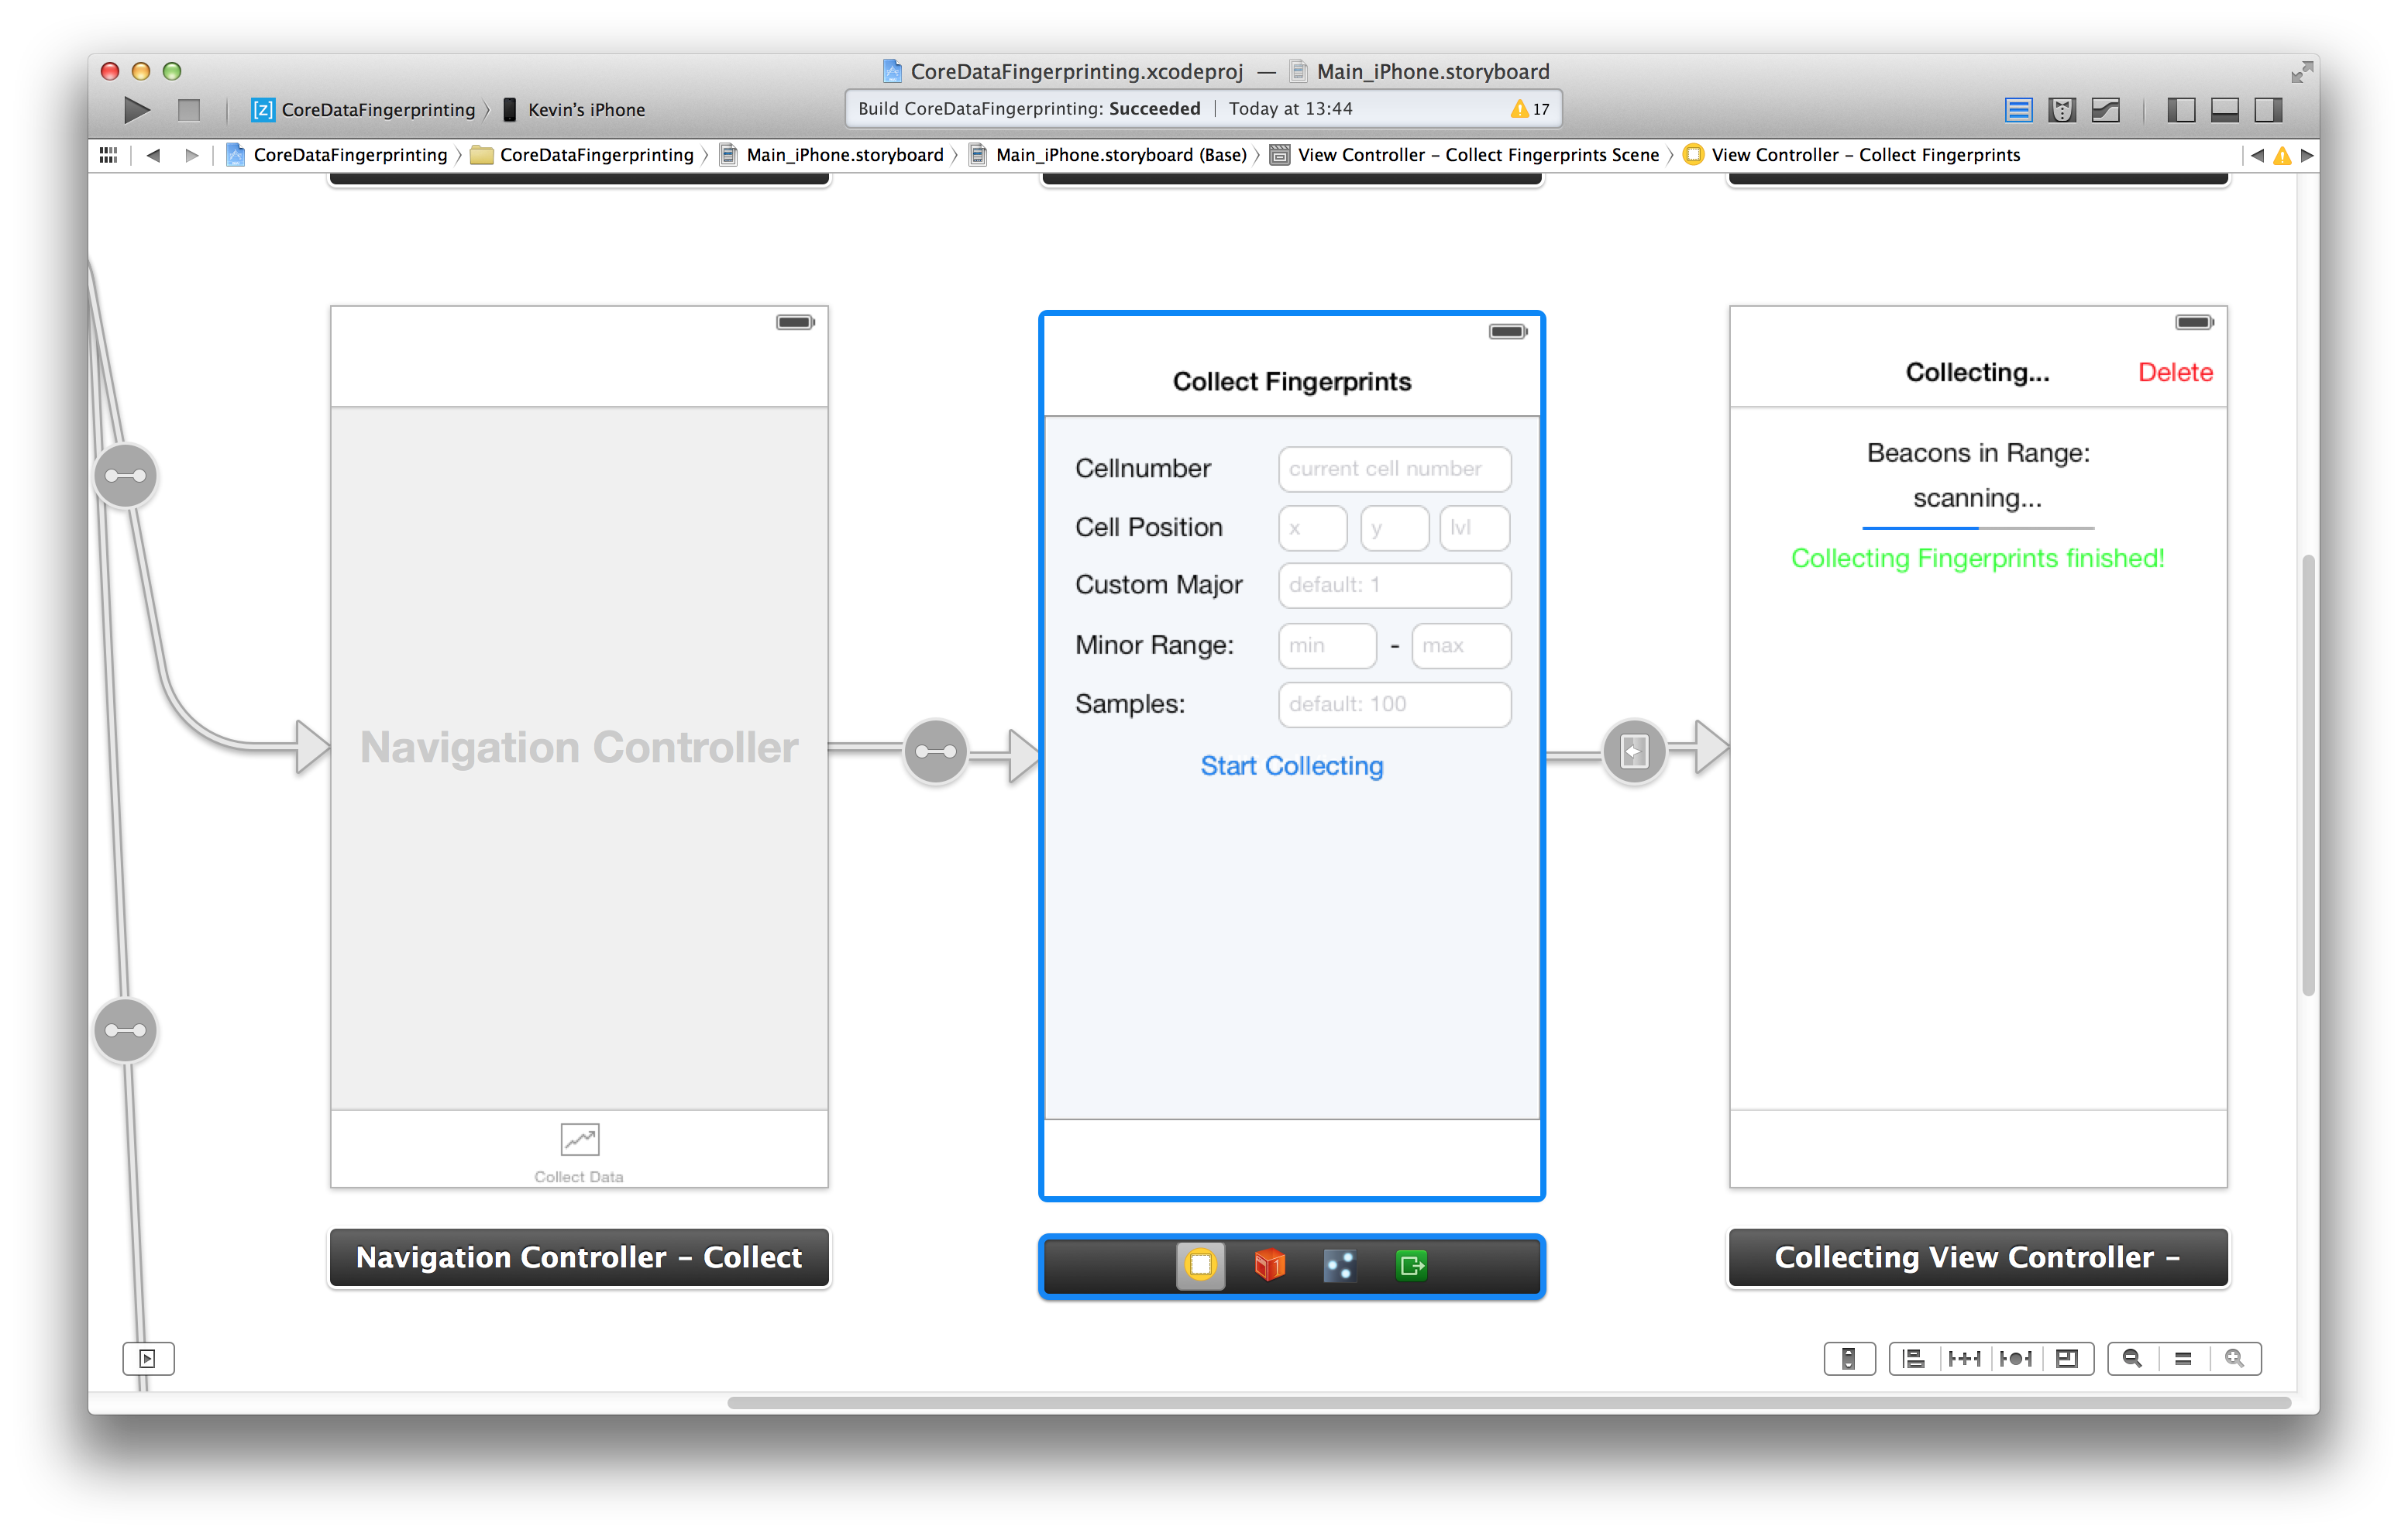
\includegraphics[scale=0.25]{xcode-storyboard}
	\caption{Beispiel eines Storyboards für iPhones}
	\label{xcode-storyboard}
\end{figure}

Das Storyboard bietet außerdem noch die Funktion des \emph{Auto Layout}. Dabei werden sogenannte \emph{Constraints} genutzt, welche die Positionsbeziehungen zwischen den einzelnen Elementen festlegen. Diese Contstraints erzeugen so ein dynamisches Interface, welches sowohl im Hochformat, als auch im Querformat ein sauberes und geordnetes Format hat.
In Abbildung \ref{xcode-storyboard-constraints} lassen sich die Abstands und Ausrichtungsbeziehungen zwischen den einzelnen Objekten gut erkennen.

\begin{figure}[htb!]
		\centering
	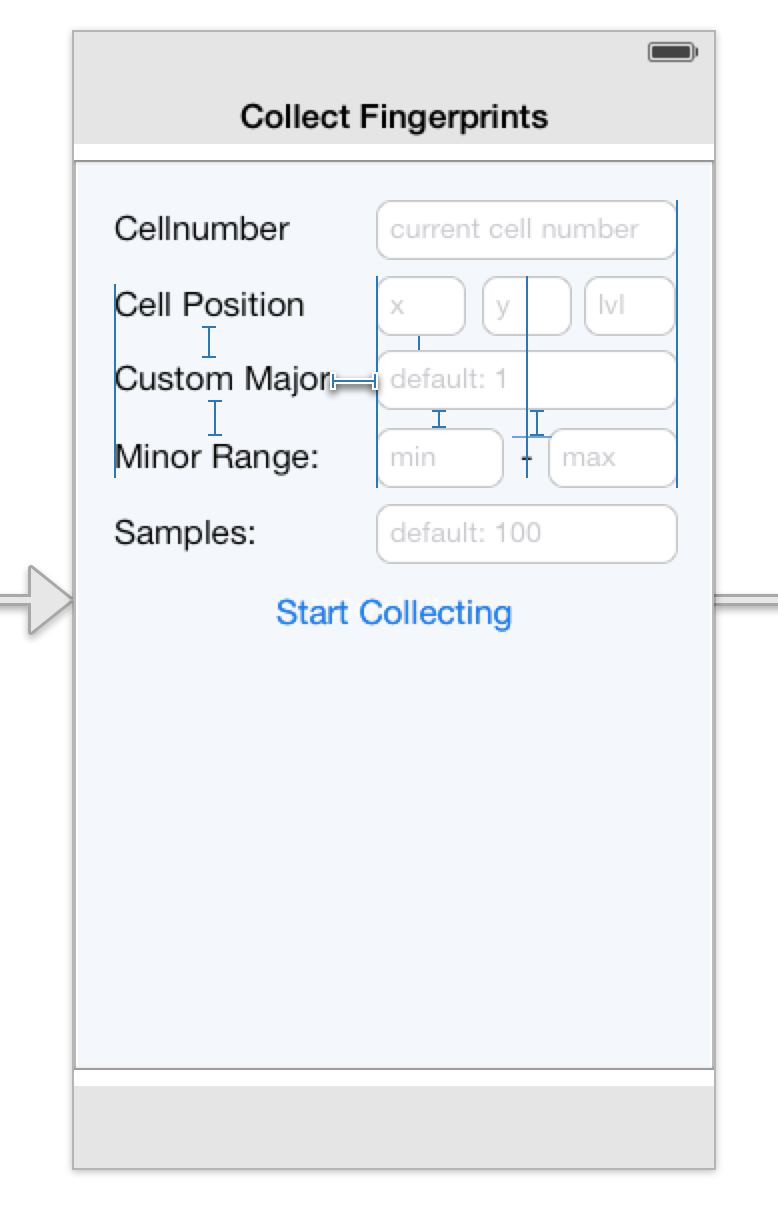
\includegraphics[scale=0.5]{xcode-storyboard-constraints}
	\caption{View Controller mit Constraints}
	\label{xcode-storyboard-constraints}
\end{figure}
\todo{Aufgabe der Constraints beschreiben}

%%%%%%%%%%%%%%%%%%%%%%%%%%%%%%%%%%%%%%%%%%%%%%%%%%%%%%%%%%%%
\section{Objective-C}
\label{sec:tools:objectivec}
%%%%%%%%%%%%%%%%%%%%%%%%%%%%%%%%%%%%%%%%%%%%%%%%%%%%%%%%%%%%
Objective-C ist eine Programmiersprache, welche in den 80er Jahren entwickelt worden ist. Sie ist eine strikte Obermenge von C und erweitert diese um objektorientierte Konzepte. Objective-C ist die Hauptsprache für die Programmierung von Cocoa-Applikationen, wie sie unter iOS und OS X genutzt werden.



%%%%%%%%%%%%%%%%%%%%%%%%%%%%%%%%%%%%%%%%%%%%%%%%%%%%%%%%%%%%
\section{Versionsverwaltung mit Git}
\label{sec:tools:git}
%%%%%%%%%%%%%%%%%%%%%%%%%%%%%%%%%%%%%%%%%%%%%%%%%%%%%%%%%%%%

%%%%%%%%%%%%%%%%%%%%%%%%%%%%%%%%%%%%%%%%%%%%%%%%%%%%%%%%%%%%
\section{iOS Developer Program}
\label{sec:iosdevprogram}
%%%%%%%%%%%%%%%%%%%%%%%%%%%%%%%%%%%%%%%%%%%%%%%%%%%%%%%%%%%%

%%%%%%%%%%%%%%%%%%%%%%%%%%%%%%%%%%%%%%%%%%%%%%%%%%%%%%%%%%%%
\section{iPhone}
\label{sec:tools:iphone}
%%%%%%%%%%%%%%%%%%%%%%%%%%%%%%%%%%%%%%%%%%%%%%%%%%%%%%%%%%%%